 \documentclass[a4paper]{article}

%NOTE BY DIRK: 	Gelieve paragrafen gewoon in te typen, geen \par gedoe.
%								Citaties liefst in de vorm "author:1999" met author=achternaam van de eerste auteur
%								figuren, tabellen, listings, ... met prefixen: fig, tab, lst, ...


\author{Olivier Berghmans, Nick De Frangh, Dirk Delahaye,\\Kristof Overdulve, Pieter-Jan Pintens, Tobias Van Bladel}
\title{Architectuur en Algoritmen van Computer Games\\\textbf{Hovercraft Universe}\\\small{\url{http://uhasseltaacgua.googlecode.com/}}}
\pagestyle{plain}
\usepackage[dutch]{babel}
\usepackage{amsfonts}
\usepackage{graphicx}
\usepackage{url}
\usepackage{todonotes}
\usepackage{hyperref}
\usepackage{parskip}
\hypersetup{
%    bookmarks=true,         % show bookmarks bar?
    unicode=false,          % non-Latin characters in Acrobat�s bookmarks
    pdftoolbar=true,        % show Acrobat�s toolbar?
    pdfmenubar=true,        % show Acrobat�s menu?
    pdffitwindow=false,     % window fit to page when opened
    pdfstartview={FitH},    % fits the width of the page to the window
    pdftitle={Architectuur en Algoritmen van Computer Games},    % title
    pdfauthor={Olivier Berghmans, Nick De Frangh, Dirk Delahaye, Kristof Overdulve, Pieter-Jan Pintens, Tobias Van Bladel},     % author
    pdfsubject={Hovercraft Universe},   % subject of the document
    %pdfcreator={Creator},   % creator of the document
    %pdfproducer={Producer}, % producer of the document
    %pdfkeywords={keywords}, % list of keywords
    pdfnewwindow=true,      % links in new window
    colorlinks=true,       % false: boxed links; true: colored links
    linkcolor=black,          % color of internal links
    citecolor=green,        % color of links to bibliography
    filecolor=magenta,      % color of file links
    urlcolor=cyan           % color of external links
}

\begin{document}

\maketitle

\tableofcontents
\newpage

\section{Introductie}

\section{Gebruikte libraries}
\begin{itemize}
\item[\textbf{Rendering}] Ogre\footnote{\url{http://www.ogre3d.org/}}
\item[\textbf{Physics}] Havok-Physics\footnote{\url{http://www.havok.com/index.php?page=havok-physics}}
\item[\textbf{Netwerk}] ZoidCom\footnote{\url{http://www.zoidcom.com/}}
\item[\textbf{Input}] Object Oriented Input System (OIS)\footnote{\url{http://sourceforge.net/projects/wgois/}}
\item[\textbf{Geluid}] FMOD Interactive Audio Middelware\footnote{\url{http://www.fmod.org/}}
\item[\textbf{Scripting}] Lua\footnote{\url{http://www.lua.org/}} en LuaBind\footnote{\url{http://www.rasterbar.com/products/luabind.html}}
\item[\textbf{GUI}] Adobe Flash\footnote{\url{http://www.adobe.com/products/flash/}} en Hikari\footnote{\url{http://code.google.com/p/hikari-library/}}.
\end{itemize}

\section{Programmastructuur en -organisatie}
\subsection{Algemeen}
De basisstructuur van de engine achter Hovercraft Universe is gemaakt naar analogie met de architectuur van \emph{Shellshock: Nam '67} \cite{rouwe:2005}. Elk object in de spelwereld waarmee ge\"interageerd kan worden, wordt voorgesteld door een \verb|Entity|. Deze entiteiten worden gegroepeerd in de \verb|EntityManager|, die de entiteiten tijdens het spel kan updaten. In onze implementatie is een \verb|Entity| tevens een uitbreiding van \verb|NetworkEntity|, die replicatie over het netwerk mogelijk maakt.

Entiteiten kunnen bestuurd worden door \verb|Controller|s. Een controller generereert \emph{events}, die door de entiteiten gepolld worden. Deze interface laat toe om entiteiten te besturen op verschillende manieren: toetsenbord/muis, AI, \ldots.

Voor de visuele representatie op de clients heeft elke relevante entiteit een \verb|EntityRepresentation|. Deze verbindt de conceptuele entiteit met een entiteit in Ogre. Om de wereld te kunnen tekenen vanuit het standpunt van \'e\'en speler worden deze representatie-objecten, samen met de Ogre camera, bijgehouden in een \verb|GameView|. 


\begin{figure}
	\centering
		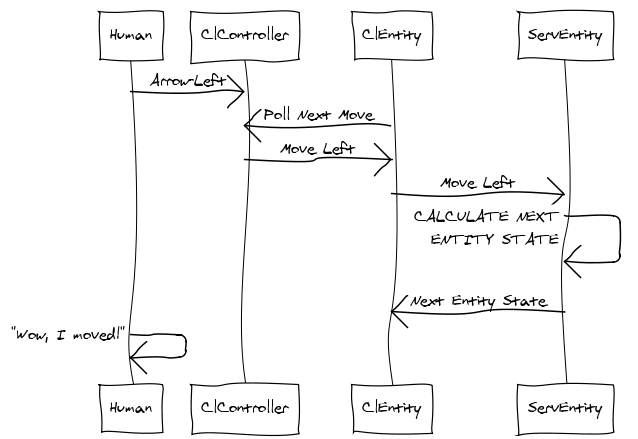
\includegraphics[width=0.50\textwidth]{images/netwerkfreq.png}
	\caption{The client entity polls its next move from the controller}
	\label{fig:netwerkfreq}
\end{figure}

\subsection{Besturing}


\subsection{Netwerkstructuur}
\begin{figure}
	\centering
		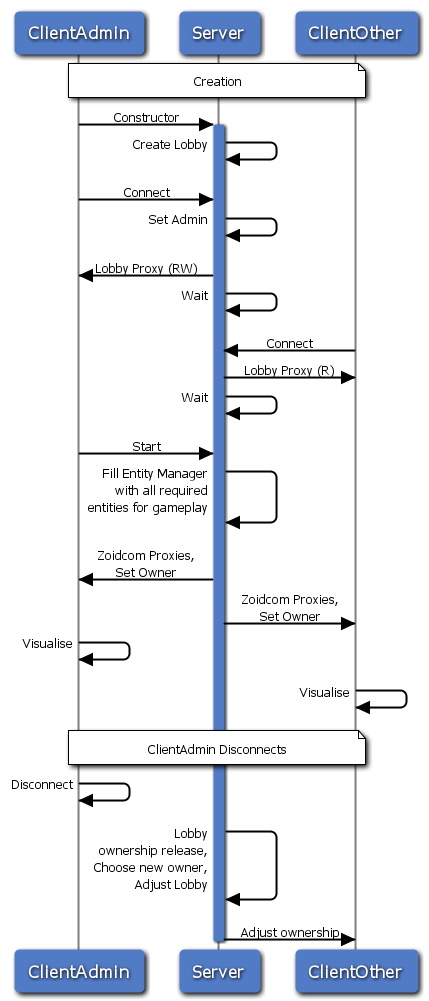
\includegraphics[width=0.50\textwidth]{images/zoidcom.png}
	\caption{ZoidCom werking}
	\label{fig:zoidcom}
\end{figure}
\todo{Over ZoidCom en het repliceren van data over het netwerk.}

\subsection{Scritping en AI}
Voor de bots is een AI voorzien, die ``menselijk'' stuurgedrag nabootst. De algoritmen van deze AI zijn gebaseerd op de autonome stuursimulaties van Craig Reynolds \cite{reynolds:1999}. De huidige AI is in staat om een voorgedefinieerd pad te volgen binnen een bepaalde marge (``Path Following''). Een pad wordt voorgesteld als een \emph{multiline}: een lijst van punten in de wereld, telkens geassocieerd met een straal (\verb|radius|). De straal op punt $x_i$ stelt de \emph{breedte} van het pad voor tussen punt $x_i$ e, $x_{i+1}$. Deze paden worden opgeslagen in aparte bestanden. Dit betekent dat de level designers per map een ideaal pad (of meerdere paden) voor de AI kunnen aanmaken. 

De AI is geprogrammeerd in Lua \cite{lerusalimschy:2006}, om aanpassing van de AI-algoritmen mogelijk te maken zonder dat het spel hiervoor gehercompileerd moet worden. Voor de binding tussen Lua en C++ wordt Luabind gebruikt. De \verb|ScriptWrapper| klasse abstraheert deze scripts en laat de programmeurs toe om met de scripts te werken, zonder Lua-specifieke constructies te moeten gebruiken.

\emph{Collision avoidance} voor de AI is ook ge\"implementeerd met behulp van Havok physics. Er zijn twee implementaties beschikbaar voor de \verb|EntityCollision| interface. Het eenvoudige model (zie Figuur~\ref{fig:simplecollisionavoidance}) plaatst een kubus op een bepaalde afstand van het voertuig om objecten te detecteren. Dit model gebruikt zeer weinig resources, maar is ook niet zo krachtig. Het geavanceerde model gebruikt een 3D-lichaam dat zich uitstrekt van het voertuig tot de gewenste afstand voor de figuur (zie Figuur~\ref{fig:advancedcollisionavoidance}). Deze manier van werken heeft een kleine meerkost in resources in vergelijking met het eenvoudige model.

Aangezien deze methodes afhankelijk zijn van de physics, draaien ze op de server. Als een object wordt gedetecteerd, wordt dit door middel van een event doorgegeven aan een callback functie in de entiteit. Dit wordt vertaald naar een boolean in de entiteit, die door het netwerk wordt gerepliceerd op de client. Client-side maakt de AI dan een beslissing om het obstakel te ontwijken.

\begin{figure}%
\begin{center}
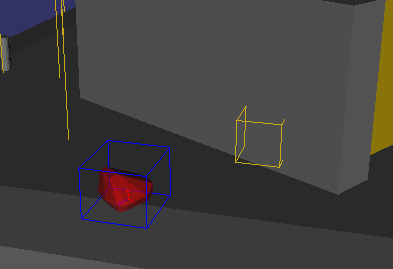
\includegraphics[width=0.4 \columnwidth]{images/collision_prevention_simple.jpg}%
\end{center}
\caption{Het eenvoudige collision avoidance model}%
\label{fig:simplecollisionavoidance}%
\end{figure}

\begin{figure}%
\begin{center}
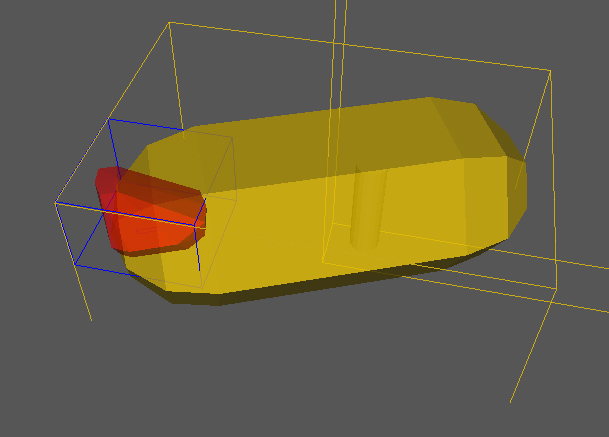
\includegraphics[width=0.8 \columnwidth]{images/collision_prevention_advanced.jpg}%
\end{center}
\caption{Het geavanceerde collision avoidance model}%
\label{fig:advancedcollisionavoidance}%
\end{figure}

\section{Rolverdeling en verantwoordelijkheden}
\todo{Of niet? :D}

\bibliographystyle{plain}
\bibliography{references}

\end{document}
